% Generated by compendium/tools/particle_chart.py from compendium/figures/particles.json; do not edit by hand.
\clearpage
\begingroup\renewcommand{\topfraction}{0.95}\renewcommand{\bottomfraction}{0.95}\renewcommand{\textfraction}{0.02}\renewcommand{\floatpagefraction}{0.75}\setcounter{topnumber}{3}\setcounter{bottomnumber}{3}\setcounter{totalnumber}{4}
\label{atlaspart:particle-webs}
\section*{The six genres and the conjectured webs of the Standard Model particles}\label{app:particle-webs}
\addcontentsline{toc}{section}{The six genres and the conjectured webs of the Standard Model particles}
Every link of a web has a genre, the pair of its end dimensions, written here with the larger end first. Figure~\ref{fig:genre-matrix} draws the six genres in two layers, kept apart on the page. The upper part of each cell is derived, from the axiom, the definitions and the read cap of the alpha Letter, which it obtains from one reading of the axiom’s last clause: one read fixes a link exactly when $d_1 d_2 \le 6$, so (2,2) and (3,2) are readable and the other four genres are dark, and a one-dimensional end is excluded at the axiom (theorem~\ref{box:I-1-axiom-and-the-six-definitions:9}). The band at the foot of each cell is conjectured: it names the sector of physics each genre is taken to correspond to, as in the abstract, (2,2) spacetime, (3,2) electromagnetism, (3,3) the strong interaction, (4,2) the weak interaction, (4,3) the Yukawa sector and (4,4) the Higgs, and where the genre appears in the particle webs. These names are conjectures and not results of the compendium. Of the two readable genres only (3,2) has an acting central charge. The readout of its link is the exact number of the alpha Letter, checked in Lean; that the number is $\alpha(0)$ is the Letter’s conjecture.

\begin{figure}[p]\centering
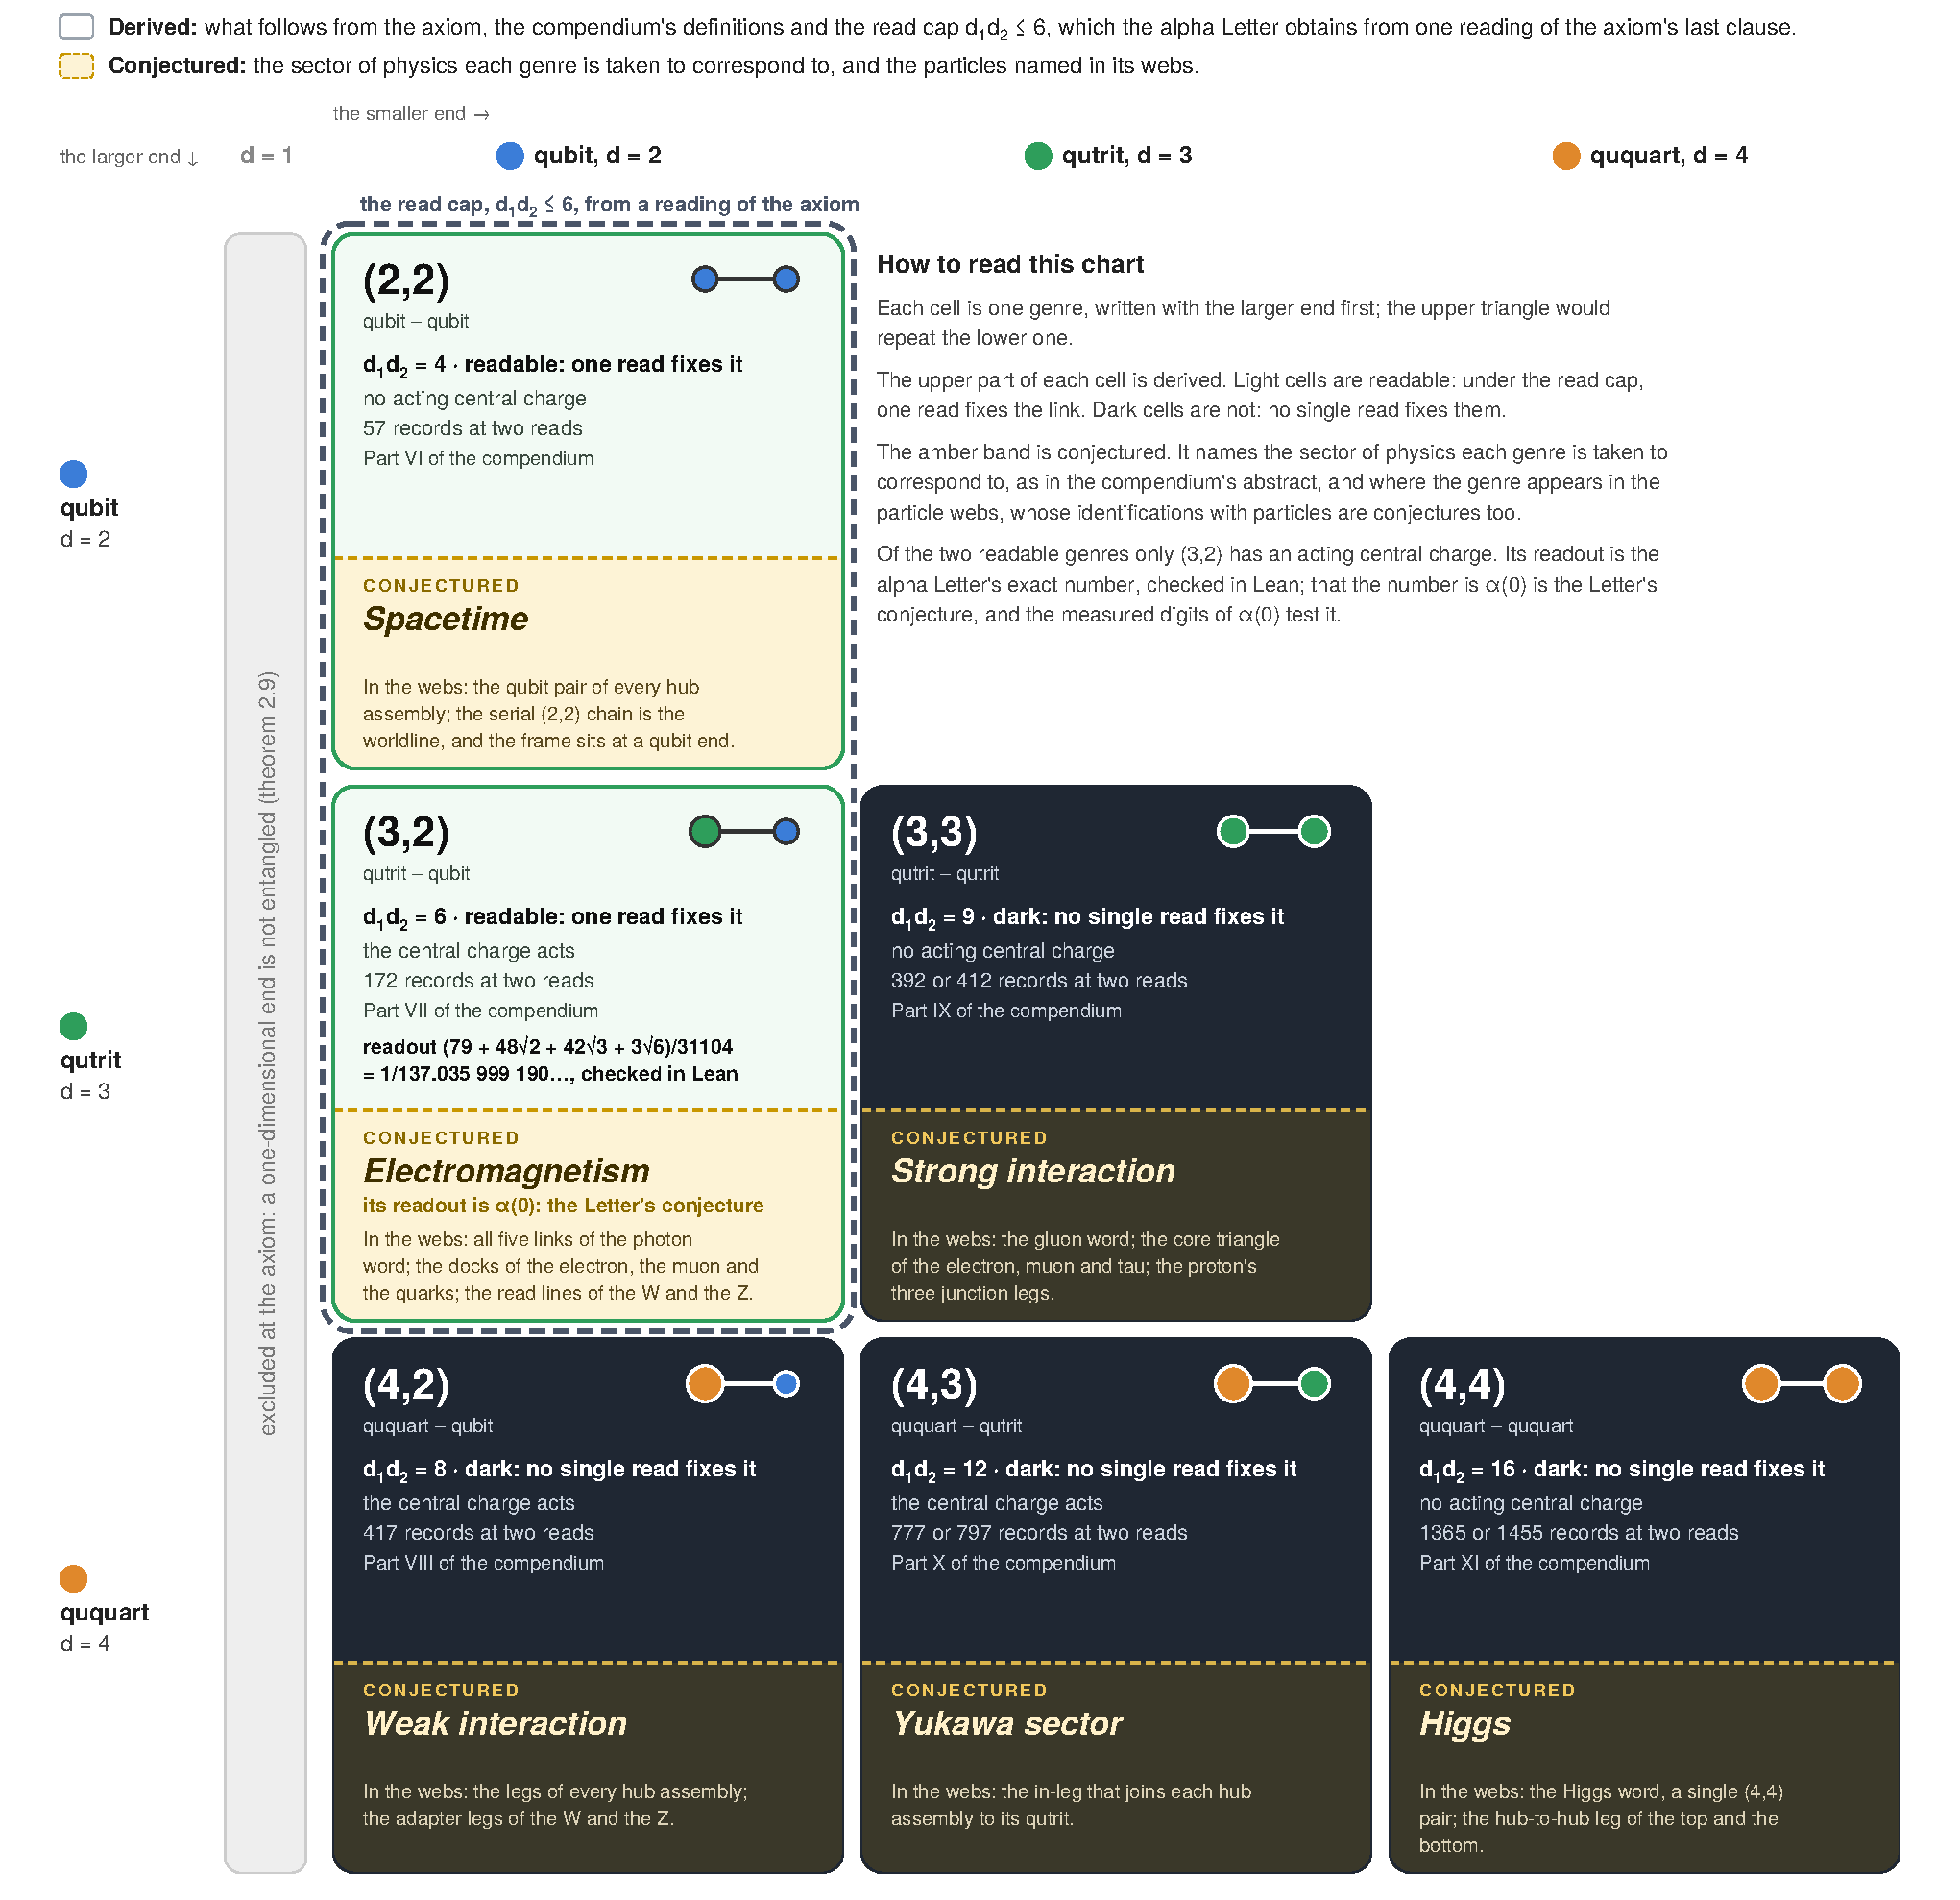
\includegraphics[width=\linewidth]{../figures/genre-matrix.pdf}
\caption{The six genres of the link, with the larger end first. The upper part of each cell is derived; the genres inside the dashed outline are readable, since one read fixes the link when $d_1 d_2 \le 6$, and the others are dark. The band at the foot of each cell is conjectured. The records are those of a link read twice; at (3,3), (4,3) and (4,4) the compendium gives two spellings of the closure sector, and both counts are shown.}\label{fig:genre-matrix}
\end{figure}

The rest of this chapter draws the web the compendium records for each Standard Model particle. That a web is the particle it is named for is a conjecture in every case. What the compendium derives is about the web, and each caption gives the standing of those results and the weakest grade among them. Every site is a qudit and every line a maximally entangled pair; the colour of a site gives its dimension (two blue, three green, four orange), a heavy ring marks a core site and a dashed ring a read site. Laid out as the Standard Model chart in Figure~\ref{fig:particle-chart}, the webs add one hub assembly at each generation. The electron is the core triangle of three qutrits with one hub assembly at a corner, and the muon and the tau carry two and three. The up quark is a qutrit with its docks, and the charm and the top add one and two hubs; the down, the strange and the bottom carry one, two and three; and the three neutrino depth webs carry one, two and three.

The W and the Z are one web, and what distinguishes them is the read: the W is read along one line and the Z along two, drawn heavy. The neutron is not drawn: its recorded body has a hub at degree five and a qutrit at degree four, beyond the valence law (at most $d$ pairs at a qudit of dimension $d$). Each identification of a web with a particle is graded where its result stands, and each figure names that standing. The layouts are for legibility and carry no content.
\begin{figure}[p]\centering
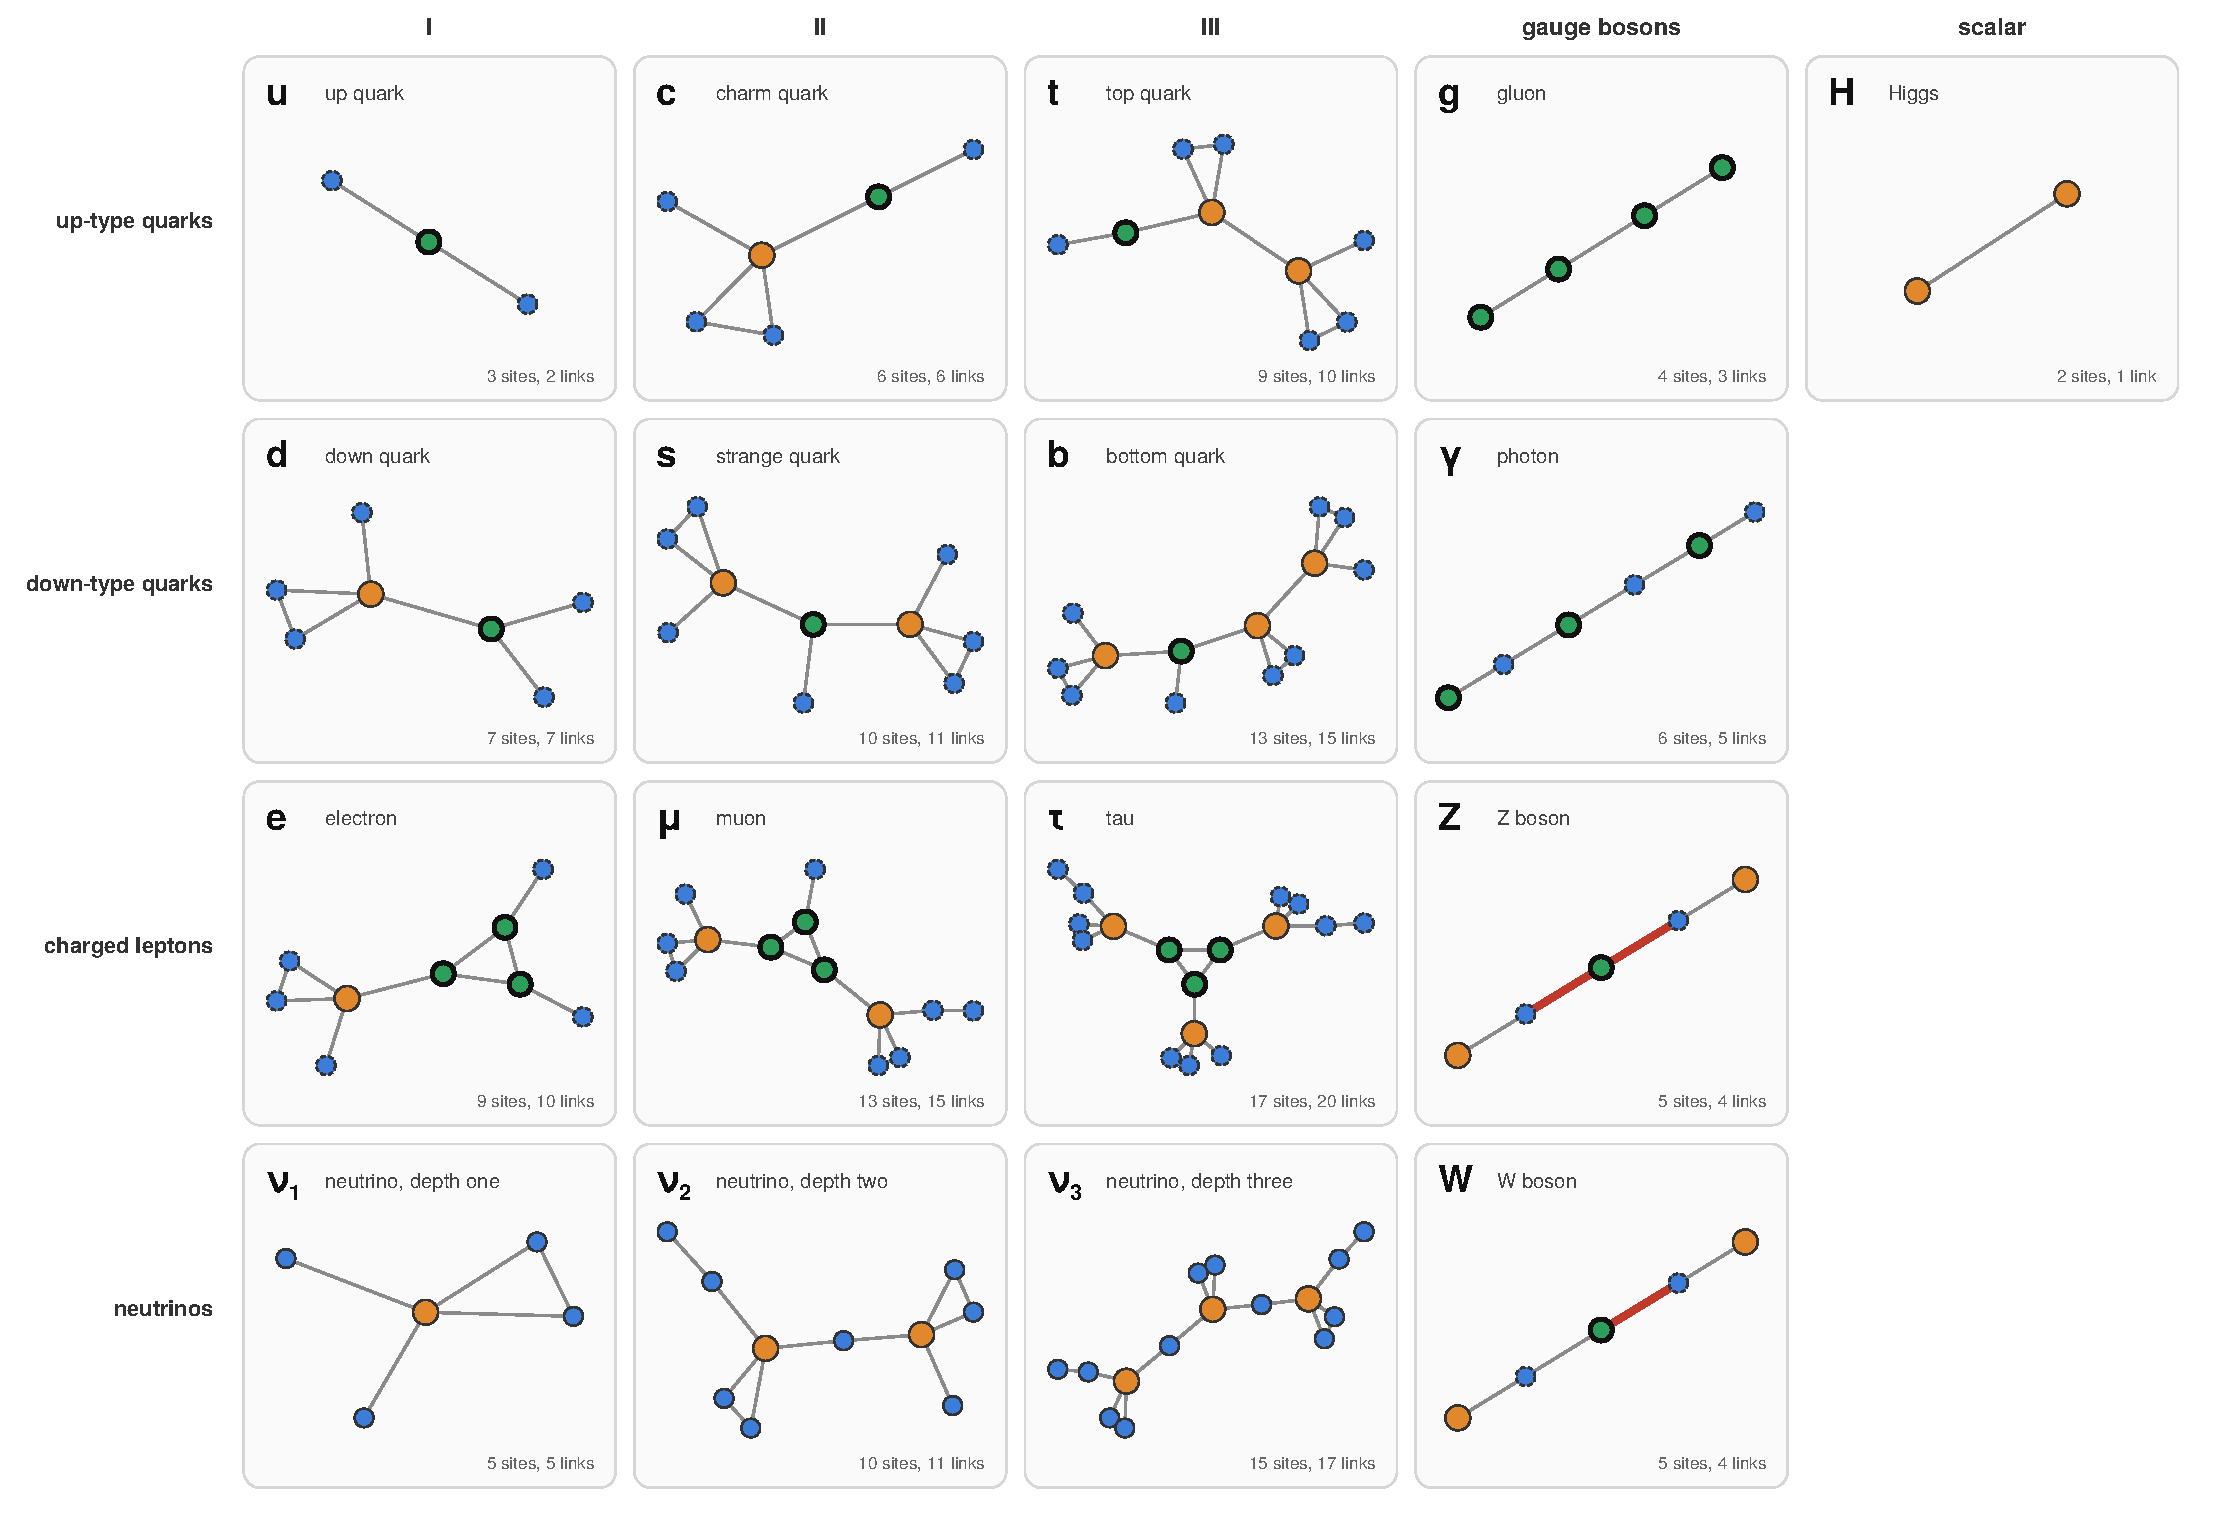
\includegraphics[width=\linewidth]{../figures/standard-model-webs.pdf}
\caption{Conjectured webs for the Standard Model particles, laid out by generation. Each generation adds one hub assembly; the W and the Z are one web, read along one line and along two.}\label{fig:particle-chart}
\end{figure}
\clearpage
\begin{figure}[htbp]\centering
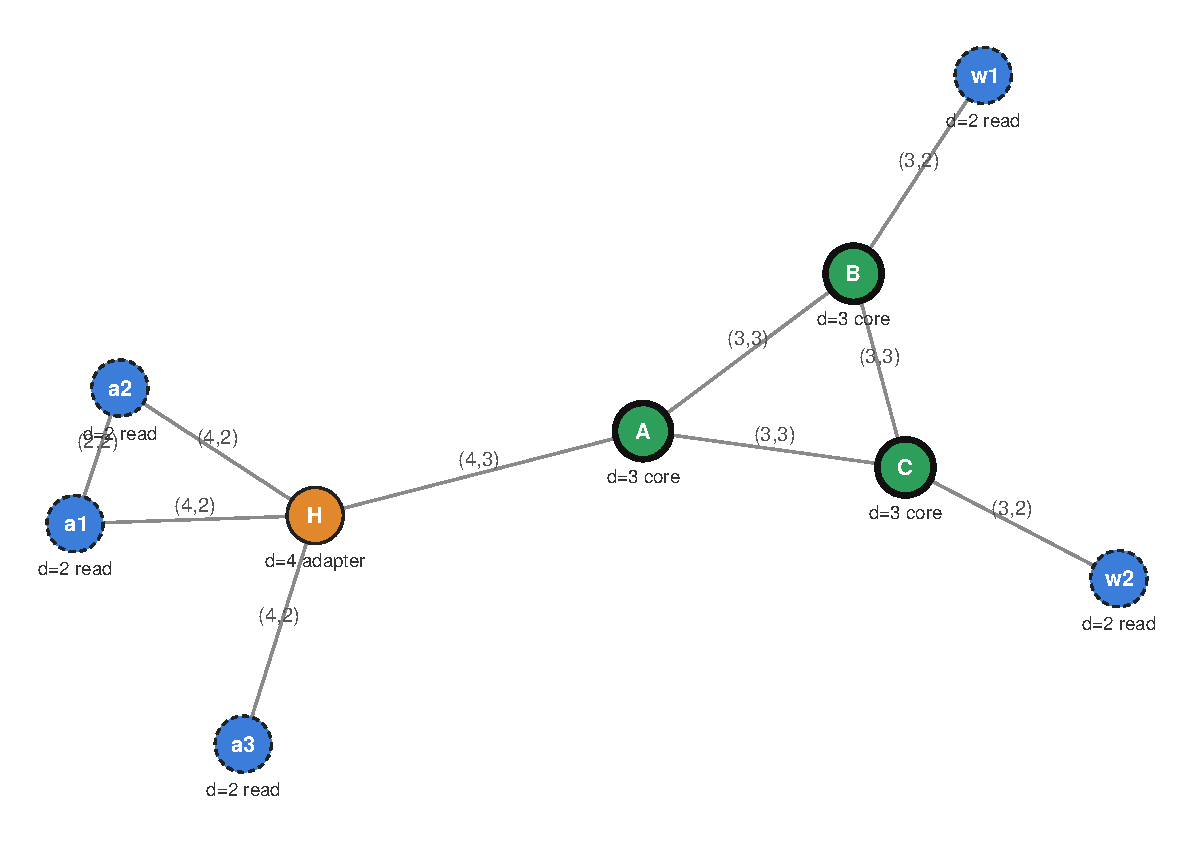
\includegraphics[width=\linewidth,height=0.36\textheight,keepaspectratio]{../figures/webs/electron.pdf}
\caption{\textbf{Electron} (e). The web \texttt{E\_TWODOCK}: 9 sites and 10 links, at the genres (2,2) 1, (3,2) 2, (3,3) 3, (4,2) 3, (4,3) 1. The lepton ladder as hub assemblies, conditional theorem 152.1: the core triangle with one hub assembly. Weakest grade: conditional theorem.}
\label{fig:particle-electron}
\end{figure}
\begin{figure}[htbp]\centering
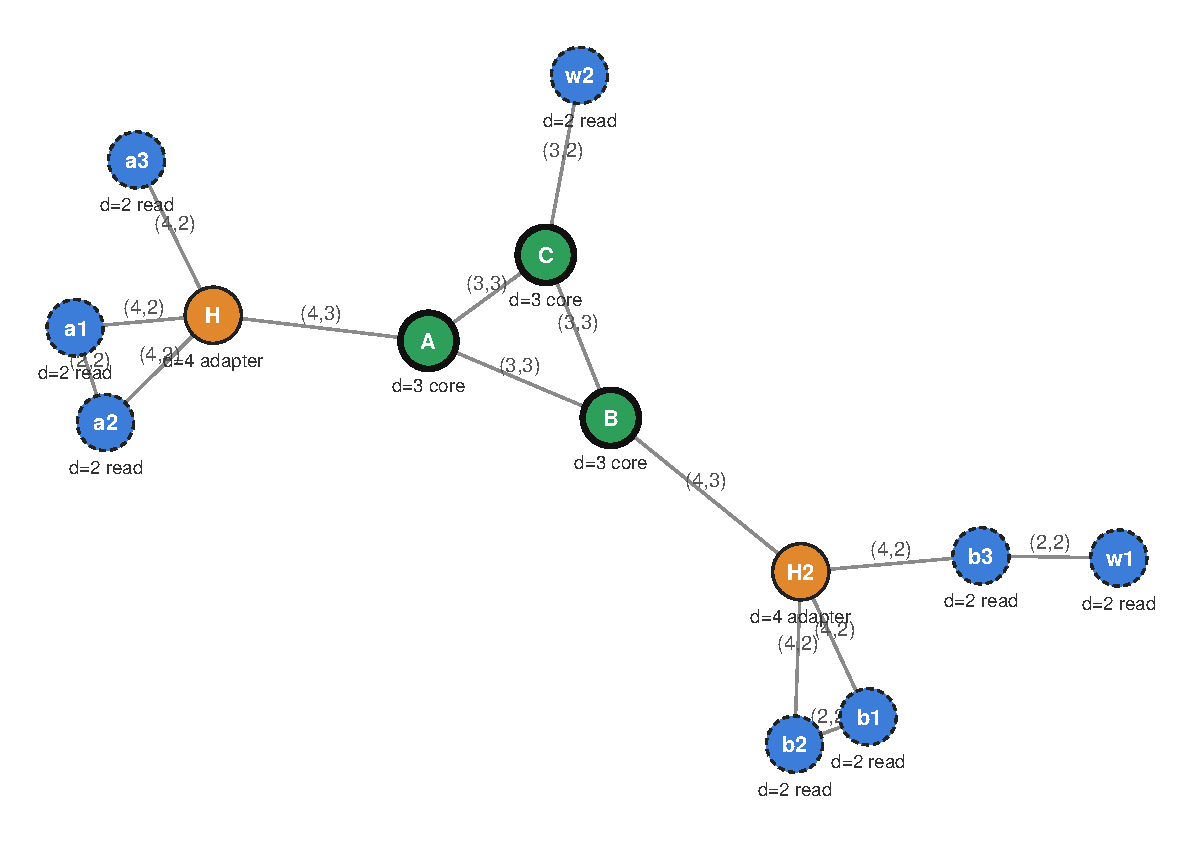
\includegraphics[width=\linewidth,height=0.36\textheight,keepaspectratio]{../figures/webs/muon.pdf}
\caption{\textbf{Muon} ($\mu$). The web \texttt{T6-MU-LEAF}: 13 sites and 15 links, at the genres (2,2) 3, (3,2) 1, (3,3) 3, (4,2) 6, (4,3) 2. The lepton ladder as hub assemblies, conditional theorem 152.1: the core triangle with two hub assemblies. Weakest grade: conditional theorem.}
\label{fig:particle-muon}
\end{figure}
\begin{figure}[htbp]\centering
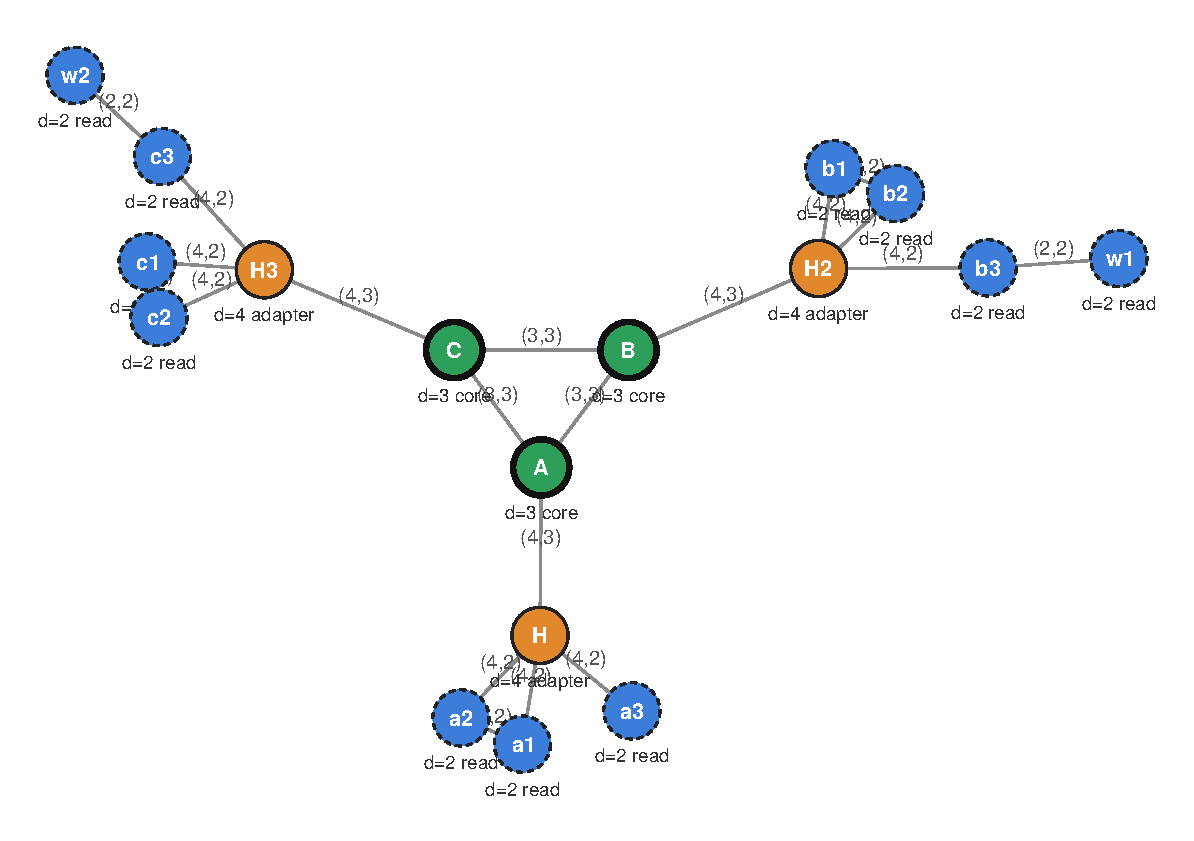
\includegraphics[width=\linewidth,height=0.36\textheight,keepaspectratio]{../figures/webs/tau.pdf}
\caption{\textbf{Tau} ($\tau$). The web \texttt{T6-TAU-LL}: 17 sites and 20 links, at the genres (2,2) 5, (3,3) 3, (4,2) 9, (4,3) 3. The tau as the third hub on the triangle core, theorem 154.1. Weakest grade: theorem.}
\label{fig:particle-tau}
\end{figure}
\begin{figure}[htbp]\centering
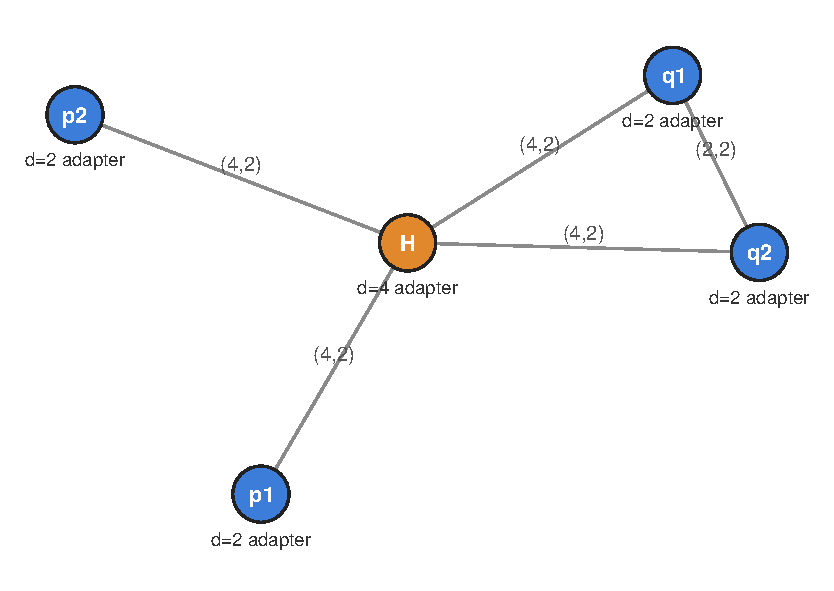
\includegraphics[width=\linewidth,height=0.36\textheight,keepaspectratio]{../figures/webs/neutrino-depth-web-n0-the-cross-core-body.pdf}
\caption{\textbf{The neutrino at depth one} ($\nu_1$). The web \texttt{CROSS-CORE-N0}: 5 sites and 5 links, at the genres (2,2) 1, (4,2) 4. The cross-core body at depth one. Its reading as a neutrino is open; the neutral sinks census is conditional theorem 162.2, and the other candidate webs are open. Weakest grade: open result.}
\label{fig:particle-neutrino-depth-web-n0-the-cross-core-body}
\end{figure}
\begin{figure}[htbp]\centering
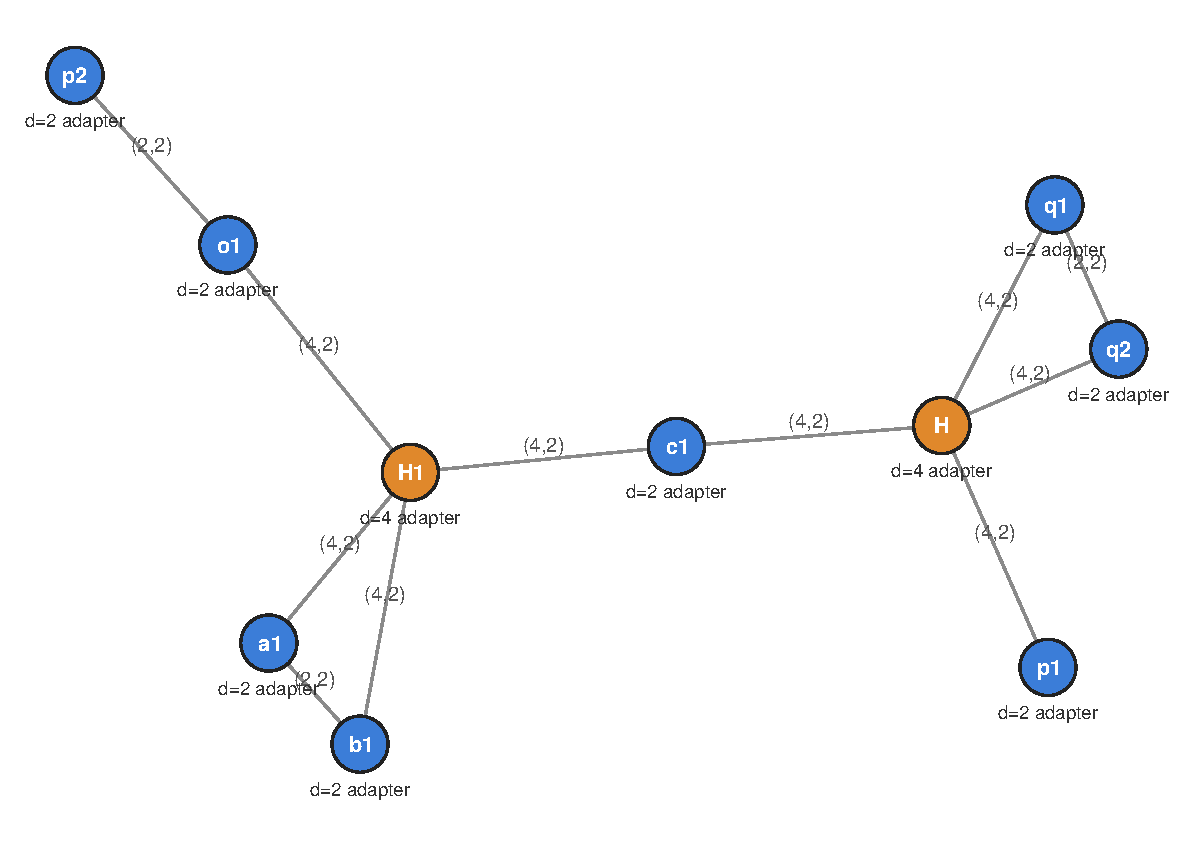
\includegraphics[width=\linewidth,height=0.36\textheight,keepaspectratio]{../figures/webs/neutrino-depth-web-n1-the-cross-core-body.pdf}
\caption{\textbf{The neutrino at depth two} ($\nu_2$). The web \texttt{CROSS-CORE-N1}: 10 sites and 11 links, at the genres (2,2) 3, (4,2) 8. The cross-core body at depth two; standing as for the first. Weakest grade: open result.}
\label{fig:particle-neutrino-depth-web-n1-the-cross-core-body}
\end{figure}
\begin{figure}[htbp]\centering
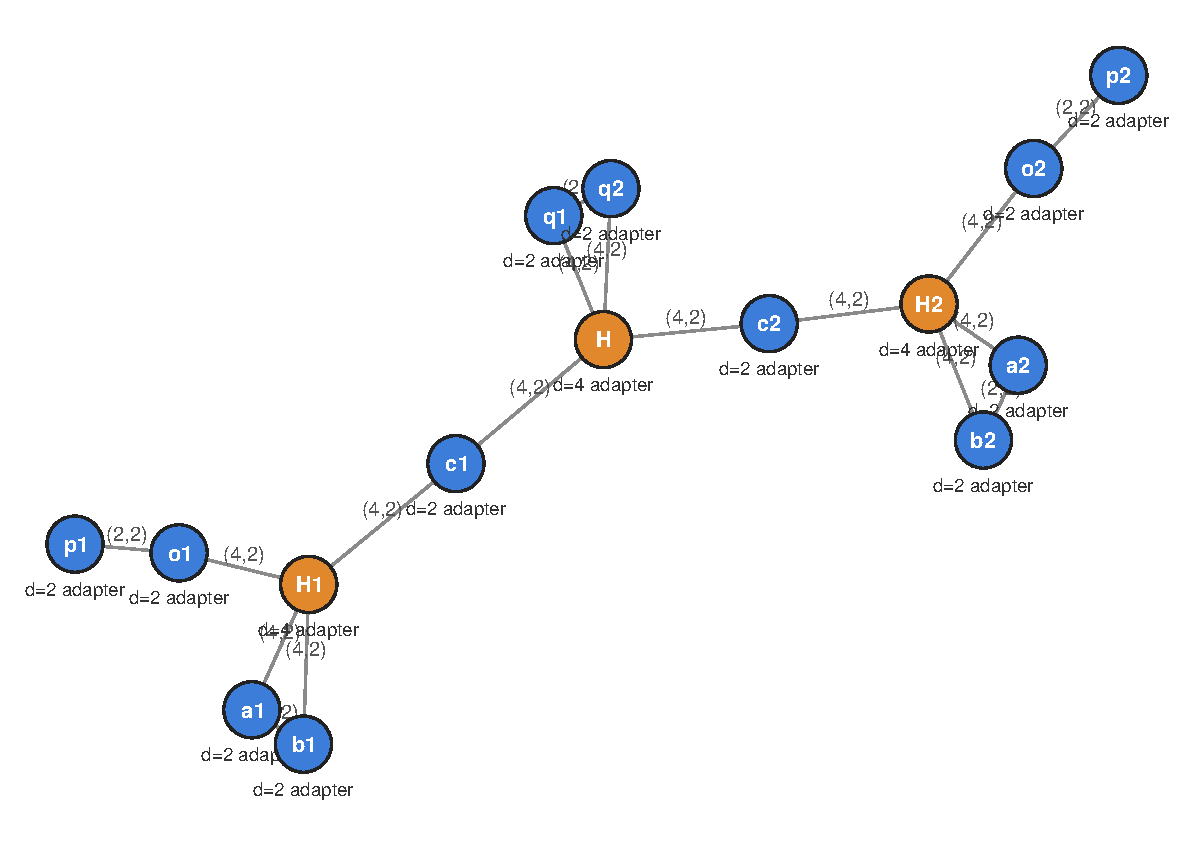
\includegraphics[width=\linewidth,height=0.36\textheight,keepaspectratio]{../figures/webs/neutrino-depth-web-n2-the-cross-core-body.pdf}
\caption{\textbf{The neutrino at depth three} ($\nu_3$). The web \texttt{CROSS-CORE-N2}: 15 sites and 17 links, at the genres (2,2) 5, (4,2) 12. The cross-core body at depth three; standing as for the first. Weakest grade: open result.}
\label{fig:particle-neutrino-depth-web-n2-the-cross-core-body}
\end{figure}
\begin{figure}[htbp]\centering
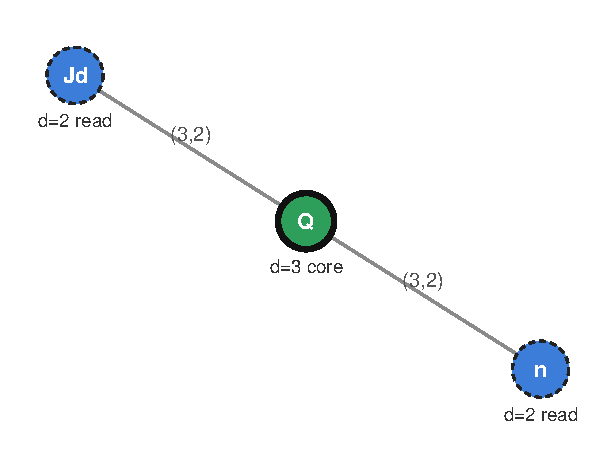
\includegraphics[width=\linewidth,height=0.36\textheight,keepaspectratio]{../figures/webs/up-quark.pdf}
\caption{\textbf{Up quark} (u). The web \texttt{U\_DOCKED}: 3 sites and 2 links, at the genres (3,2) 2. Flavor as the rung name and the quark ladder, conditional theorem 181.2. Weakest grade: conditional theorem.}
\label{fig:particle-up-quark}
\end{figure}
\begin{figure}[htbp]\centering
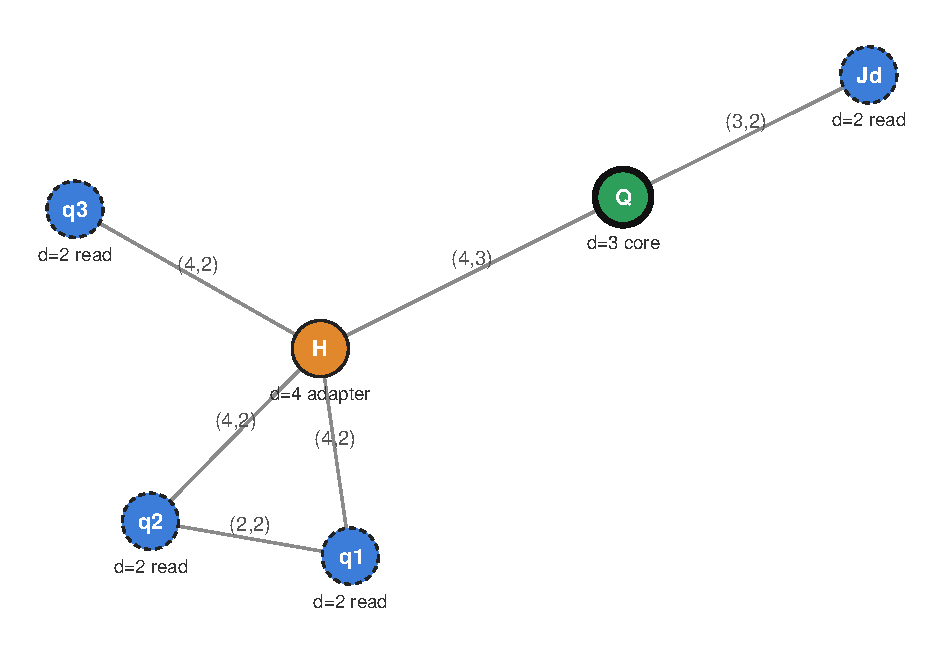
\includegraphics[width=\linewidth,height=0.36\textheight,keepaspectratio]{../figures/webs/charm-quark.pdf}
\caption{\textbf{Charm quark} (c). The web \texttt{C\_DOCKED}: 6 sites and 6 links, at the genres (2,2) 1, (3,2) 1, (4,2) 3, (4,3) 1. The quark ladder, conditional theorems 181.2 and 181.4. Weakest grade: conditional theorem.}
\label{fig:particle-charm-quark}
\end{figure}
\begin{figure}[htbp]\centering
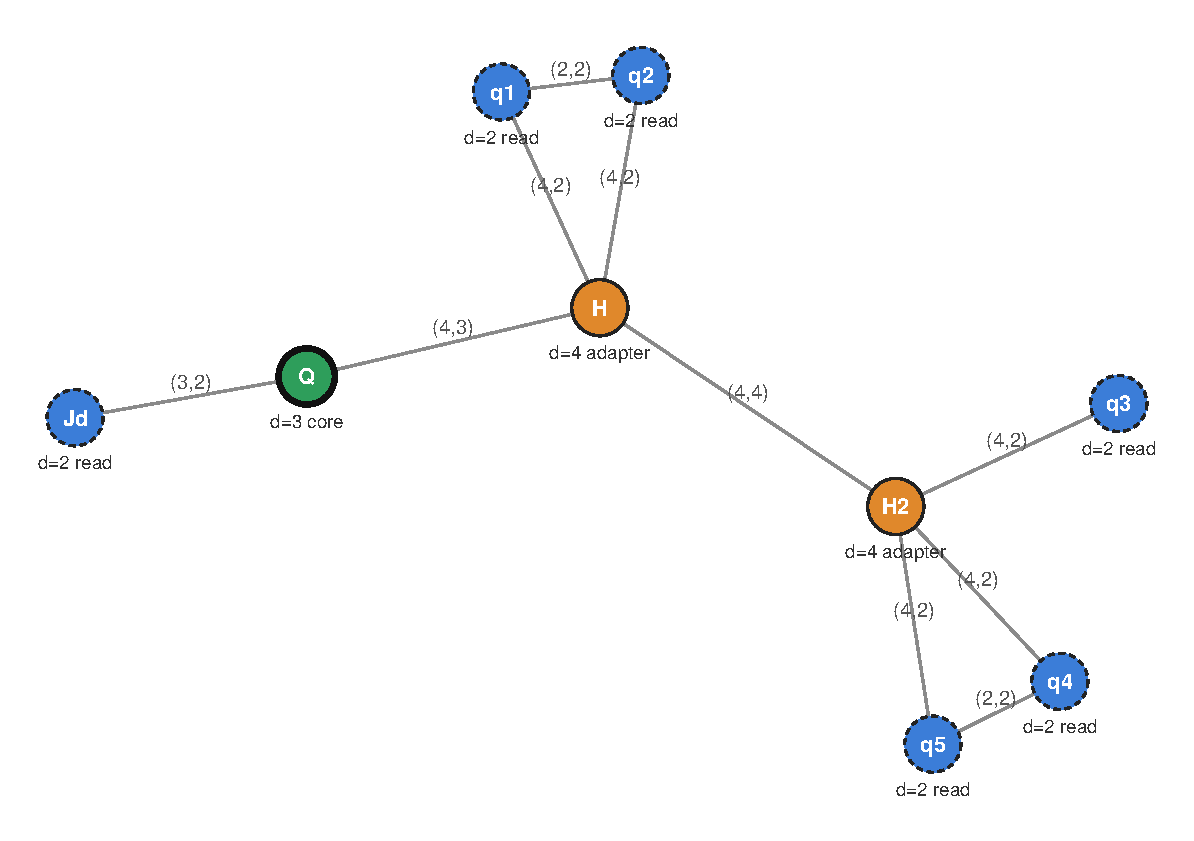
\includegraphics[width=\linewidth,height=0.36\textheight,keepaspectratio]{../figures/webs/top-quark.pdf}
\caption{\textbf{Top quark} (t). The web \texttt{TA\_DOCKED}: 9 sites and 10 links, at the genres (2,2) 2, (3,2) 1, (4,2) 5, (4,3) 1, (4,4) 1. The quark ladder, conditional theorems 181.2 and 181.4. Weakest grade: conditional theorem.}
\label{fig:particle-top-quark}
\end{figure}
\begin{figure}[htbp]\centering
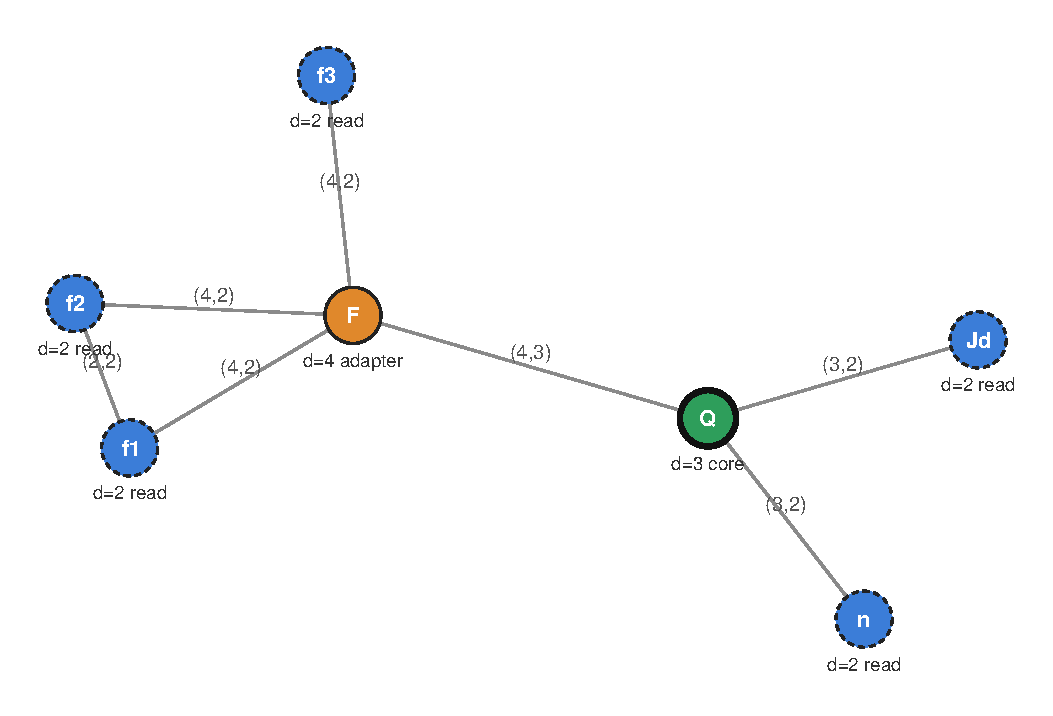
\includegraphics[width=\linewidth,height=0.36\textheight,keepaspectratio]{../figures/webs/down-quark.pdf}
\caption{\textbf{Down quark} (d). The web \texttt{D\_DOCKED}: 7 sites and 7 links, at the genres (2,2) 1, (3,2) 2, (4,2) 3, (4,3) 1. The quark ladder, conditional theorems 181.2 and 181.4. Weakest grade: conditional theorem.}
\label{fig:particle-down-quark}
\end{figure}
\begin{figure}[htbp]\centering
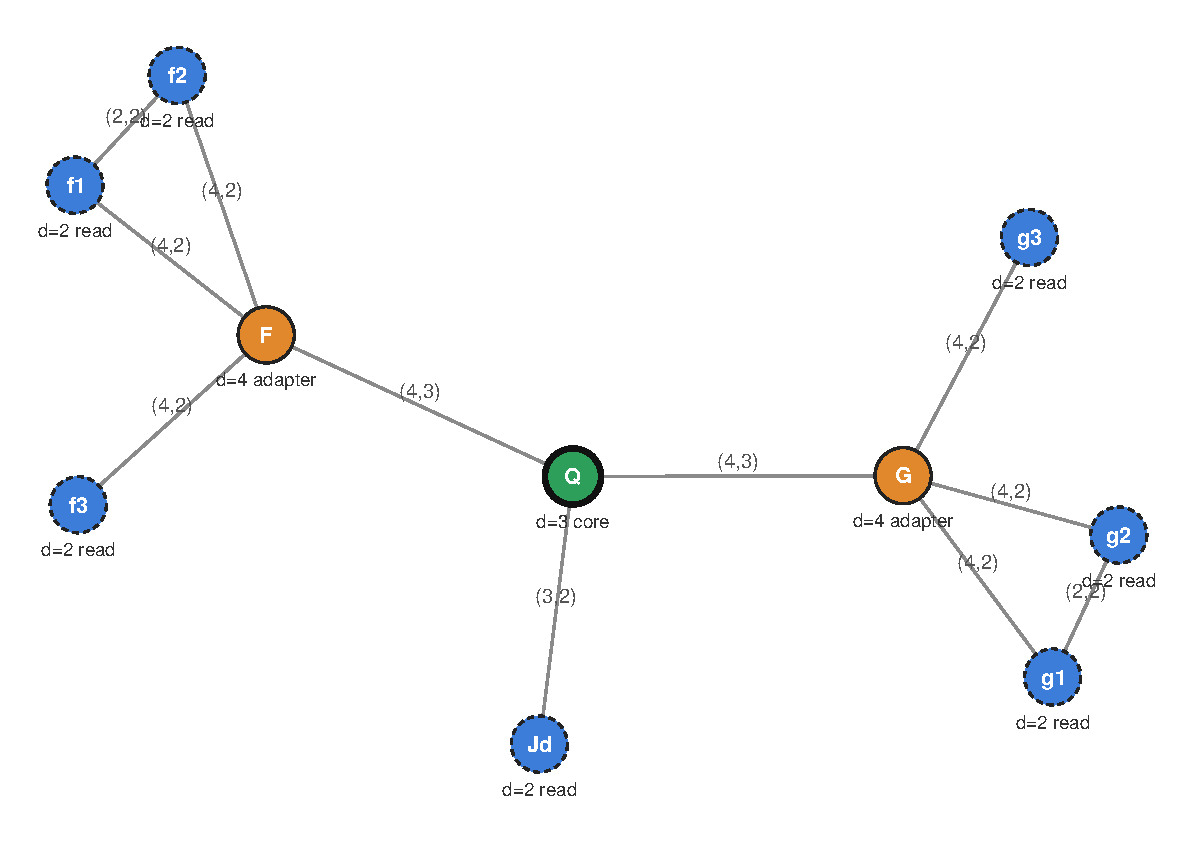
\includegraphics[width=\linewidth,height=0.36\textheight,keepaspectratio]{../figures/webs/strange-quark.pdf}
\caption{\textbf{Strange quark} (s). The web \texttt{S\_DOCKED}: 10 sites and 11 links, at the genres (2,2) 2, (3,2) 1, (4,2) 6, (4,3) 2. The quark ladder, conditional theorems 181.2 and 181.4. Weakest grade: conditional theorem.}
\label{fig:particle-strange-quark}
\end{figure}
\begin{figure}[htbp]\centering
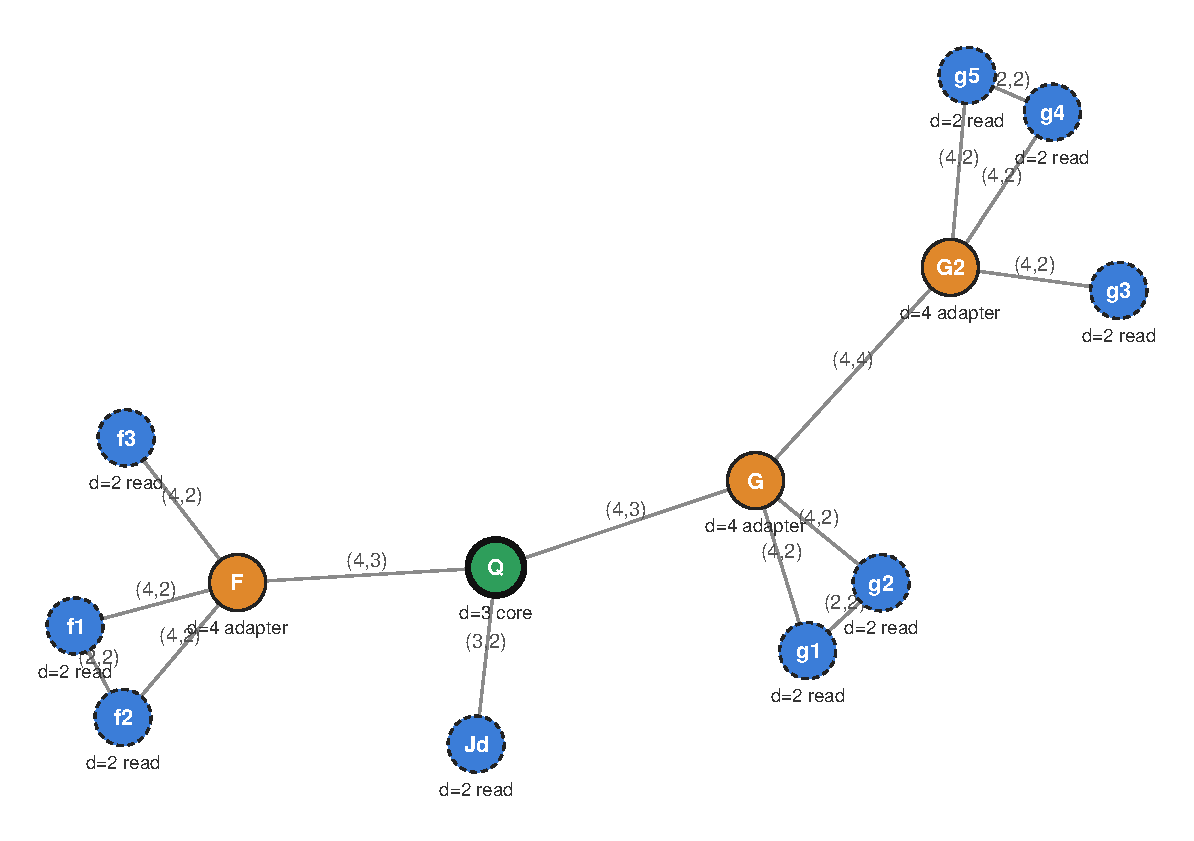
\includegraphics[width=\linewidth,height=0.36\textheight,keepaspectratio]{../figures/webs/bottom-quark.pdf}
\caption{\textbf{Bottom quark} (b). The web \texttt{BA\_DOCKED}: 13 sites and 15 links, at the genres (2,2) 3, (3,2) 1, (4,2) 8, (4,3) 2, (4,4) 1. The quark ladder, conditional theorems 181.2 and 181.4. Weakest grade: conditional theorem.}
\label{fig:particle-bottom-quark}
\end{figure}
\begin{figure}[htbp]\centering
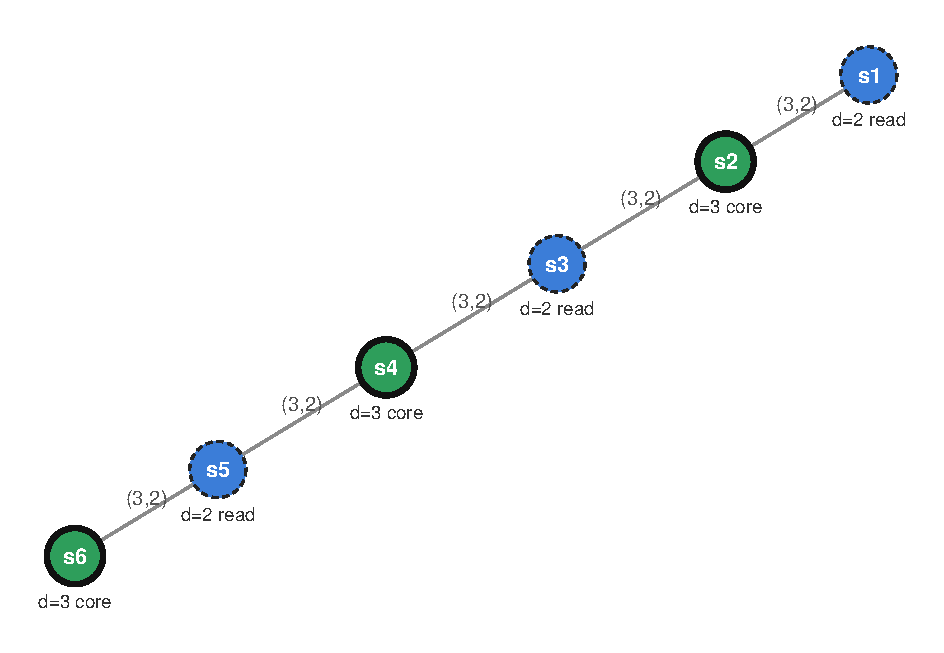
\includegraphics[width=\linewidth,height=0.36\textheight,keepaspectratio]{../figures/webs/photon.pdf}
\caption{\textbf{Photon} ($\gamma$). The web \texttt{r-GAM}: 6 sites and 5 links, at the genres (3,2) 5. The photon word. The (2,3) open link as the photon is theorem 134.1; the photon docks at both faces, conditional theorem 150.1. Weakest grade: conditional theorem.}
\label{fig:particle-photon}
\end{figure}
\begin{figure}[htbp]\centering
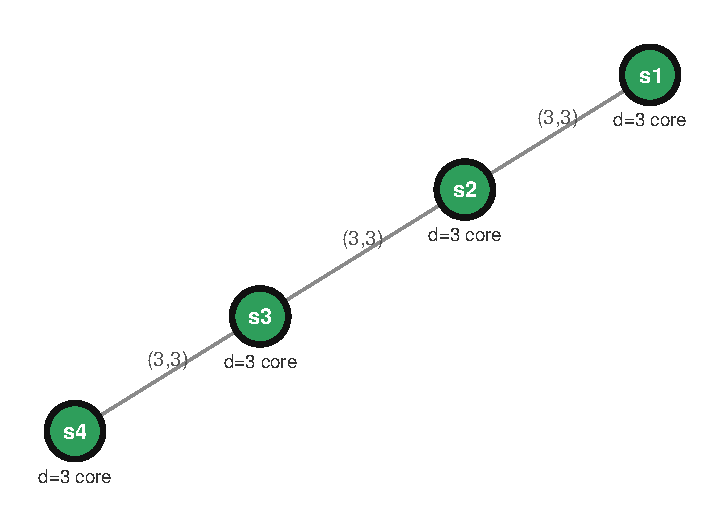
\includegraphics[width=\linewidth,height=0.36\textheight,keepaspectratio]{../figures/webs/gluon.pdf}
\caption{\textbf{Gluon} (g). The web \texttt{r-GLU}: 4 sites and 3 links, at the genres (3,3) 3. The gluon word. The strong coupling as the gluon pair-ket office is conditional theorem 149.1. Weakest grade: conditional theorem.}
\label{fig:particle-gluon}
\end{figure}
\begin{figure}[htbp]\centering
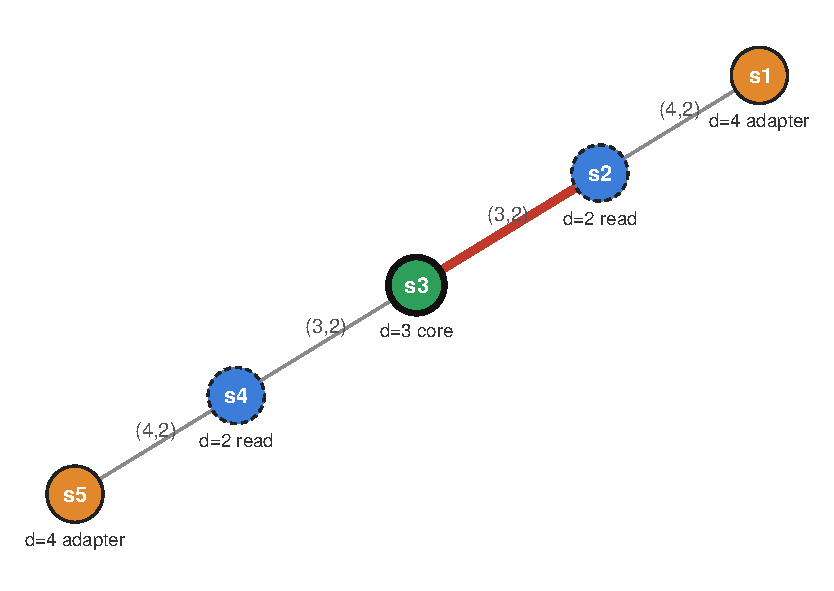
\includegraphics[width=\linewidth,height=0.36\textheight,keepaspectratio]{../figures/webs/w-boson.pdf}
\caption{\textbf{W boson} (W). The web \texttt{r-WPM}: 5 sites and 4 links, at the genres (3,2) 2, (4,2) 2. The W word, read along one line (heavy). The W word as the passage web of the cross read is open result 159.2. Weakest grade: open result.}
\label{fig:particle-w-boson}
\end{figure}
\begin{figure}[htbp]\centering
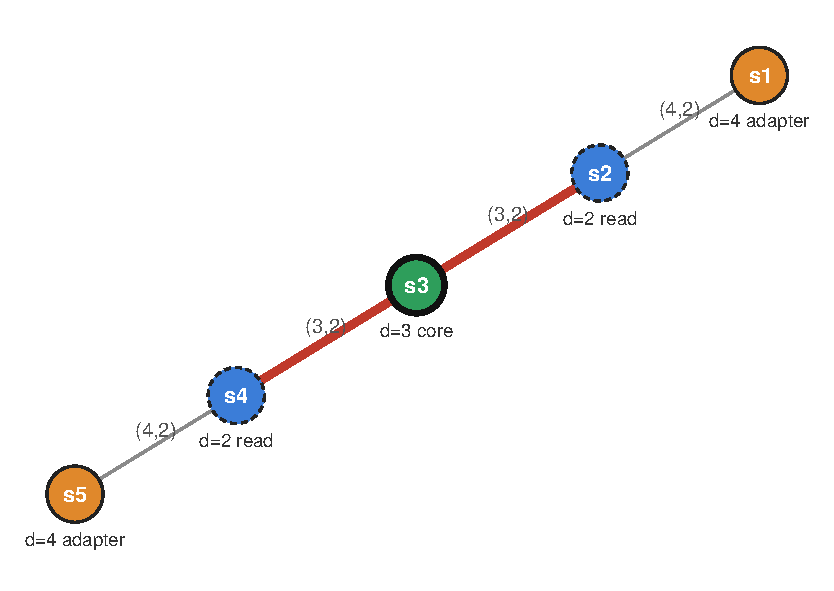
\includegraphics[width=\linewidth,height=0.36\textheight,keepaspectratio]{../figures/webs/z-boson.pdf}
\caption{\textbf{Z boson} (Z). The web \texttt{r-Z0D}: 5 sites and 4 links, at the genres (3,2) 2, (4,2) 2. The same web as the W, read along two lines (heavy): open result 159.1. The ratio of the two offices is 1/2, conditional theorem 164.5; the W over Z mass ratio is open result 160.1. Weakest grade: open result.}
\label{fig:particle-z-boson}
\end{figure}
\begin{figure}[htbp]\centering
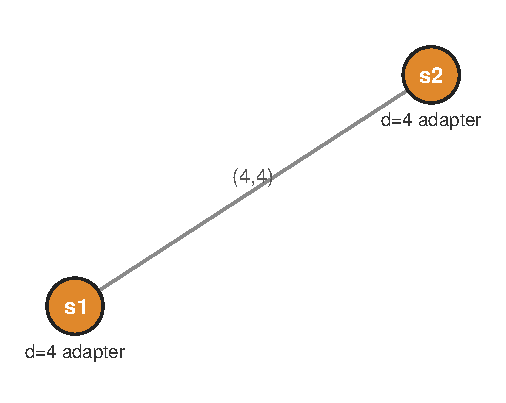
\includegraphics[width=\linewidth,height=0.36\textheight,keepaspectratio]{../figures/webs/higgs.pdf}
\caption{\textbf{Higgs} (H). The web \texttt{r-HIG}: 2 sites and 1 link, at the genres (4,4) 1. The Higgs as the closed hub read, conditional theorem 200.1. Weakest grade: conditional theorem.}
\label{fig:particle-higgs}
\end{figure}
\begin{figure}[htbp]\centering
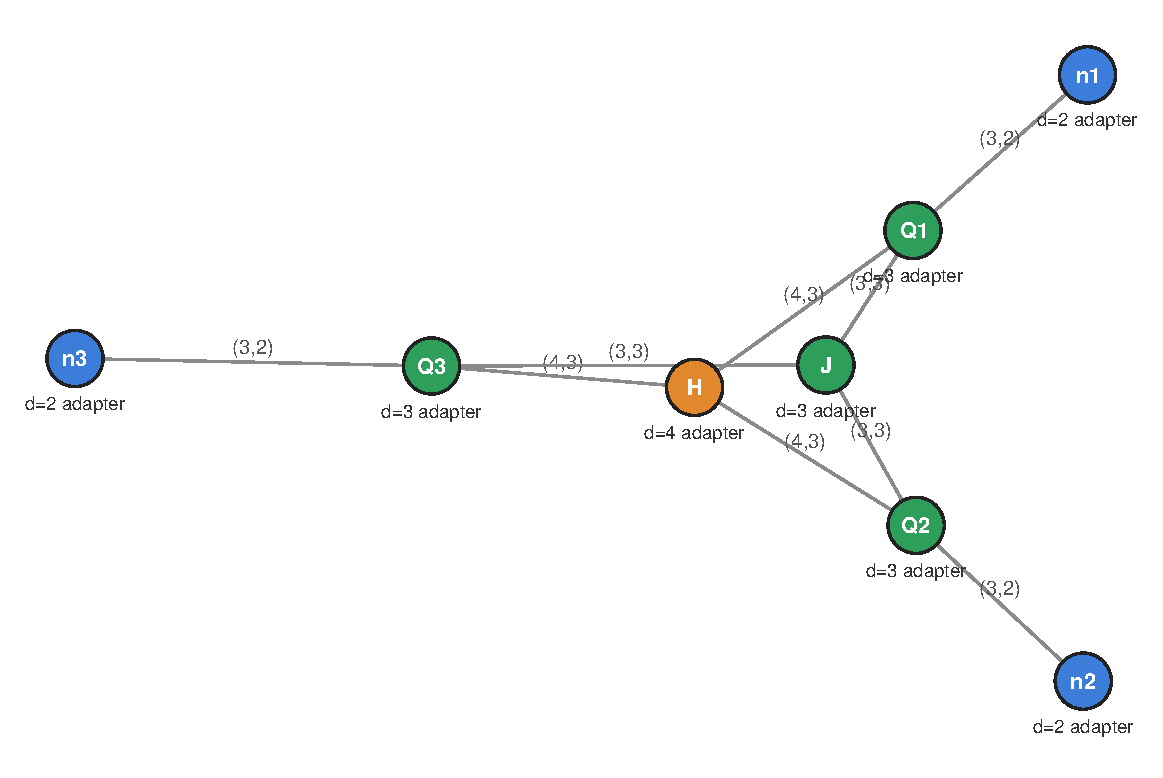
\includegraphics[width=\linewidth,height=0.36\textheight,keepaspectratio]{../figures/webs/proton-the-star-core-of-record.pdf}
\caption{\textbf{The proton} (p). The web \texttt{PROTON-SINK-NAMED}: 8 sites and 9 links, at the genres (3,2) 3, (3,3) 3, (4,3) 3. The proton as a seeded sink: the seeded saturation is open result 175.1 and the joined read at the roster stars conditional theorem 175.2. Its quark content, two ups and a down, is a reading of its three docks and is not derived. Weakest grade: open result.}
\label{fig:particle-proton-the-star-core-of-record}
\end{figure}
\begin{figure}[htbp]\centering
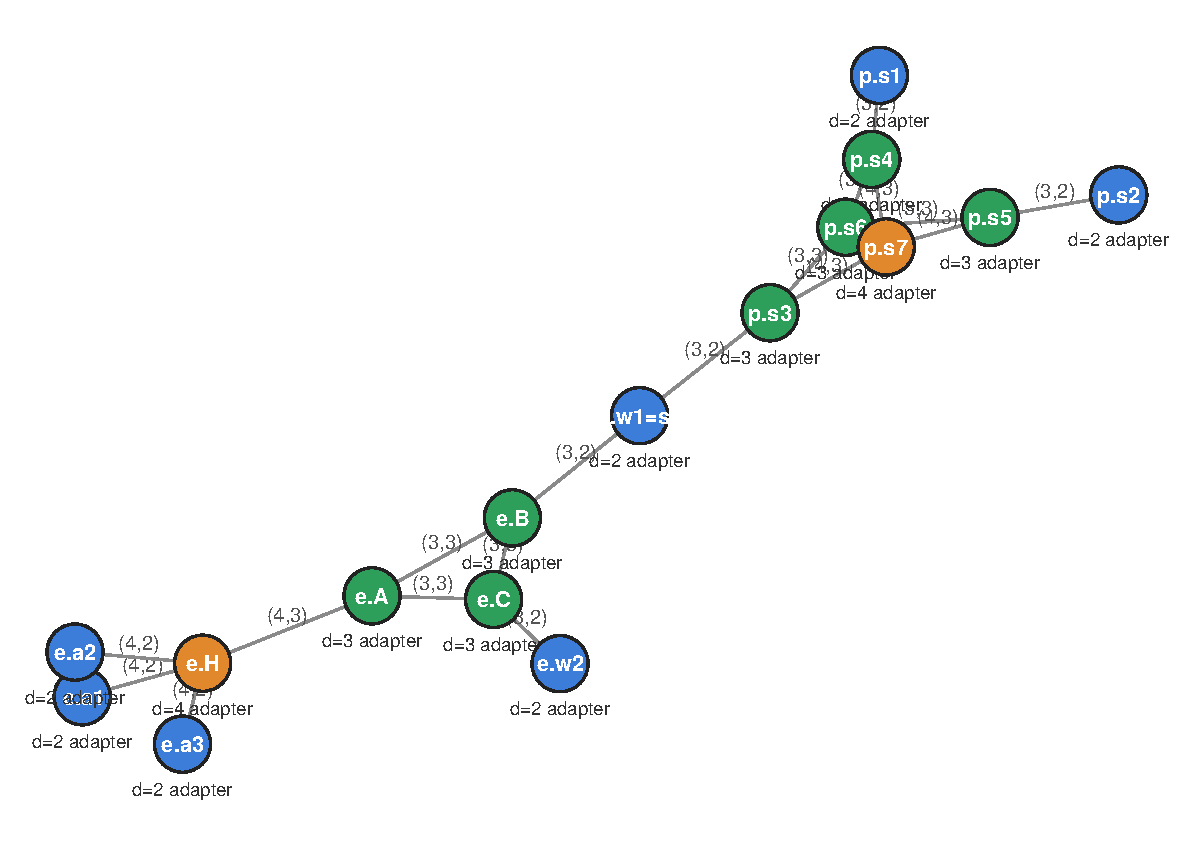
\includegraphics[width=\linewidth,height=0.36\textheight,keepaspectratio]{../figures/webs/hydrogen-the-joined-seed-ep2s1.pdf}
\caption{\textbf{Hydrogen} (H). The web \texttt{SEED-EP2S1}: 16 sites and 19 links, at the genres (2,2) 1, (3,2) 5, (3,3) 6, (4,2) 3, (4,3) 4. The electron web and the proton joined at a shared dock. Hydrogen from the held carrier is conditional theorem 143.1. Weakest grade: conditional theorem.}
\label{fig:particle-hydrogen-the-joined-seed-ep2s1}
\end{figure}
\clearpage
\endgroup
\label{atlaspart:particle-websend}
